% !TEX TS-program = pdflatex
% !TEX encoding = UTF-8 Unicode

% This is a simple template for a LaTeX document using the "article" class.
% See "book", "report", "letter" for other types of document.

\documentclass[10pt,twocolumn]{article}

\usepackage[utf8]{inputenc} % set input encoding (not needed with XeLaTeX)
\usepackage{graphicx}
\usepackage{listings} 
\usepackage{xcolor,colortbl}
\usepackage[section]{placeins}
\usepackage{amsthm}
\usepackage{mathtools}
\graphicspath{ {images/} }

%%% Examples of Article customizations
% These packages are optional, depending whether you want the features they provide.
% See the LaTeX Companion or other references for full information.

%%% PAGE DIMENSIONS
\usepackage{geometry} % to change the page dimensions
\geometry{a4paper} % or letterpaper (US) or a5paper or....
\geometry{margin=0.55in} % for example, change the margins to 2 inches all round
% \geometry{landscape} % set up the page for landscape
%   read geometry.pdf for detailed page layout information

\usepackage{graphicx} % support the \includegraphics command and options

% \usepackage[parfill]{parskip} % Activate to begin paragraphs with an empty line rather than an indent

%%% PACKAGES
\usepackage{booktabs} % for much better looking tables
\usepackage{array} % for better arrays (eg matrices) in maths
\usepackage{paralist} % very flexible & customisable lists (eg. enumerate/itemize, etc.)
\usepackage{verbatim} % adds environment for commenting out blocks of text & for better verbatim
\usepackage{subfig} % make it possible to include more than one captioned figure/table in a single float
\usepackage{indentfirst}
\usepackage{amsfonts}
\usepackage{amssymb}
\usepackage{amsthm}
% These packages are all incorporated in the memoir class to one degree or another...

%%% HEADERS & FOOTERS
\usepackage{fancyhdr} % This should be set AFTER setting up the page geometry
\pagestyle{fancy} % options: empty , plain , fancy
\renewcommand{\headrulewidth}{0pt} % customise the layout...
\lhead{}\chead{}\rhead{}
\lfoot{}\cfoot{\thepage}\rfoot{}

%%% SECTION TITLE APPEARANCE
\usepackage{sectsty}
\allsectionsfont{\sffamily\mdseries\upshape} % (See the fntguide.pdf for font help)
% (This matches ConTeXt defaults)

%%% ToC (table of contents) APPEARANCE
\usepackage[nottoc,notlof,notlot]{tocbibind} % Put the bibliography in the ToC
\usepackage[titles,subfigure]{tocloft} % Alter the style of the Table of Contents
\renewcommand{\cftsecfont}{\rmfamily\mdseries\upshape}
\renewcommand{\cftsecpagefont}{\rmfamily\mdseries\upshape} % No bold!
\setlength{\parindent}{0.5cm} 

%%% END Article customizations

%%% The "real" document content comes below...

\title{Studies on Twin Primes in Goldbach Partitions of Even Numbers}
\author{Marcin Barylski}
\date{\small{Published: November 1, 2017 \\The last update: December 29, 2018}}

\definecolor{Gray}{gray}{0.85}
\definecolor{LightCyan}{rgb}{0.88,1,1}
\newcolumntype{a}{>{\columncolor{Gray}}c}
\newcolumntype{b}{>{\columncolor{white}}c}

\newtheorem{theorem}{Theorem}
\newtheorem{lemma}[theorem]{Lemma}

\newcommand\bigforall{\mbox{\huge $\mathsurround0pt\forall$}} 
\newcommand\bigexists{\mbox{\huge $\mathsurround0pt\exists$}} 

\begin{document}
\maketitle

\begin{abstract}
Goldbach strong conjecture states that all even integers $n \textgreater 2$ can be expressed as the sum of two prime numbers (Goldbach partitions of $n$). This work is devoted to studies on twin primes present in Goldbach partitions. Based on executed experiments original Goldbach conjecture has been extended to a form that all even integers $n \textgreater 4$  can be expressed as the sum of twin prime and prime.
\end{abstract}

\section{Introduction}

Goldbach strong (also called binary) conjecture asserts that all positive even integer $n$ $\geq$ 4 can be expressed as the sum of two prime numbers. This hypothesis, formulated by Goldbach in 1742 in letter to Euler \cite{goldbach1742} and then updated by Euler to the form above is one of the oldest and still unsolved problems in number theory. Empirical verification showed that it is true for all $n$ $\leq$ 4 x $10^{18}$ \cite{oliveira2012} \cite{oliveira2013}.
The expression of a given number $n$ as a sum of two primes $p_1$ and $p_2$ is called a Goldbach Partition (GP) of $n$. Let $r(n)$ be the number of GPs of $n$ and let $R(n)$ be a set of distinct GPs of $n$ (uniqueness guaranteed through $p_1$  $\leq$ $p_2$). Goldbach strong conjecture may be rewritten that  $r(n) > 0$ for all $n \geq 4$. Computational experiments show that bottom estimation for $min(r(n))$ is increasing with $n$ (Figure $\ref{fig:pairs}$). \cite{woon2000} formulates conjecture that lower and upper bounds can be expressed as simple exponentials. \par

\begin{figure}[ht]
\centering
\captionsetup{justification=centering}
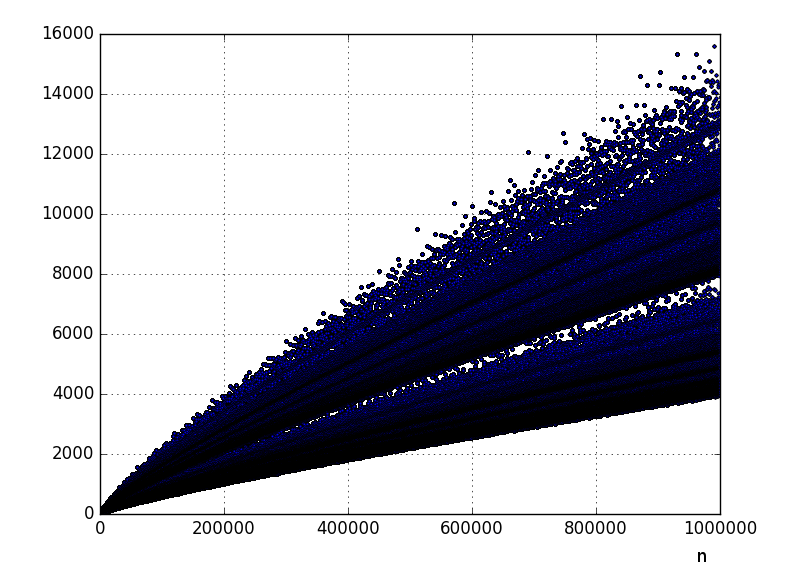
\includegraphics[width=9cm]{f_pairs}
\caption{$r(n)$ ($2$ \textless $n$ \textless $10^6$, $n = 2k, k \in \mathbb{N}$)}
\label{fig:pairs}
\end{figure}

Prime number $p$ is a twin prime if either $p-2$ or $p+2$ is another prime. Let's denote a set of twin primes as $\mathbb{P_T}$ and a set of primes as $\mathbb{P}$. OEIS A014574 \cite{A014574} lists first twin pairs of form $m \pm 1$. Twin prime conjecture, still unsolved, states that there are an infinite number of twin primes. In twin pair $(p, p+2)$ first number $p$ is called the lesser of twin primes (OEIS A001359 \cite{A001359}), $p+2$ - the greater of twin primes (OEIS A006512 \cite{A006512}). 

\begin{lemma}
$5$ is the only prime which is both the lesser of twin primes (to 7) and the greater of twin primes (to 3).
\end{lemma}
\begin{proof}
In a set of numbers $n, n+2, n+4$ one is always divisible by $3$. $n+2$ can be both the lesser of twin primes and the greater of twin primes if and only if all $n, n+2, n+4$ are primes. $3$ is the only prime which is divisible by $3$, so $3$ must be in sequence $n, n+2, n+4$. $3$ must be the first number of the sequence, because two other combinations: $1, 3, 5$ and $-1, 1, 3$ are not containing primes only. This means that the only allowed sequence is $3, 5, 7$ and $5$ is the only prime which is a member of two distinct twin primes $(3, 5)$ and $(5, 7)$. 
\end{proof}

\section{Primality tests}

For the sake of this work, to check if a given number is prime or not, algorithm skewed in Listing 1 was used. Presented approach is taking advantage of preloaded prime and composite sets (containing prime and composite numbers found earlier) which gives instant result. Then, algorithm is testing if a candidate for prime is even (divides it by $2$) or is a multiple of $3$ - in case of success the candidate is confirmed as a composite number. Eventually, it is taking advantage of Lemma 2.

\lstset{language=Python}
\lstset{breaklines=true}
\lstset{frame=shadowbox}
\lstset{caption={Primality test}}
\begin{lstlisting}[linewidth=8.7cm]
# in: integer n
#   prime_set - a set of primes
#   composite_set - a set of non-primes
# out: True if n is prime; False otherwise
def  is_prime (n):
  if n<=1:
    return False
  elsif n<=3:
    return True
  elsif n in prime_set:
    return True
  elsif n in composite_set:
    return False
  elsif n%2 == 0 or n%3 == 0:
    return False
  i=5
  while i*i<=n:
    if n%i == 0 or n%(i+2) == 0:
      return False
     i+=6
  return True
\end{lstlisting}

Listing 2 presents a simplified method how to classify a given prime number as a part of twin prime pair, including criterion for either the lesser or the greater of twin primes.

\begin{figure}[!ht]
\centering
\captionsetup{justification=centering}
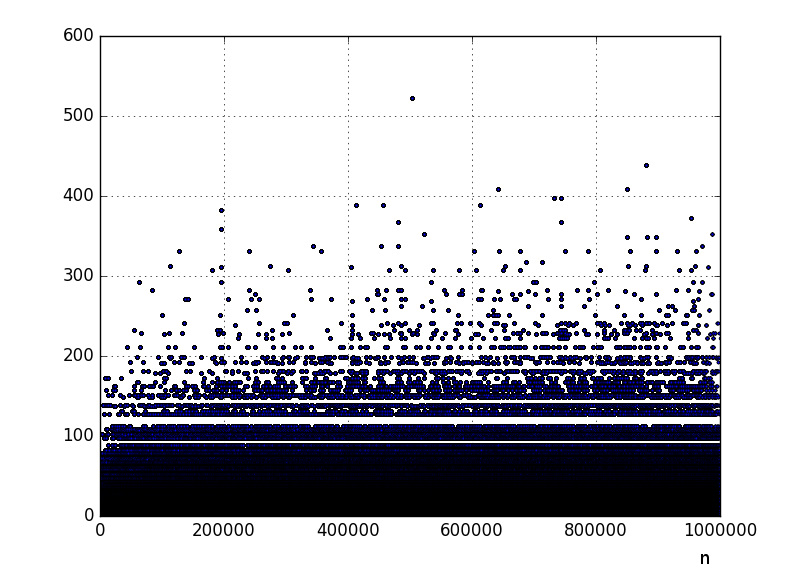
\includegraphics[width=9cm]{f_min_prime_in_sum}
\caption{Minimal prime in $R(n)$ \\ ($2$ \textless $n$ \textless $10^6$, $n = 2k, k \in \mathbb{N}$)}
\label{fig:minprime}
\end{figure}

\lstset{language=Python}
\lstset{breaklines=true}
\lstset{frame=shadowbox}
\lstset{caption={Tests for twin primes}}
\begin{lstlisting}[linewidth=8.7cm]
# in: integer n
# external dependencies:
#      is_prime() method
# out: True if n is twin prime; 
#      False otherwise
def  is_twin_prime (p):
  if n in twinprime_set:
    return True
  elsif n in composite_set:
    return False
  if is_greater_twin_prime (p) or is_lesser_twin_prime (p):
     return True
  return False

# in: integer n
# out: True if n is the greater of twin primes;
#      False otherwise
def  is_greater_twin_prime (p):
  if is_prime (p) and is_prime (p-2):
     return True
  return False
  
# in: integer n
# out: True if n is the lesser of twin primes; 
#      False otherwise
def  is_lesser_twin_prime (p):
  if is_prime (p) and is_prime (p+2):
     return True
  return False
\end{lstlisting}

\begin{lemma}
Every prime $p \textgreater 3$ can be written as $p=6k \pm 1$ (where $k$ is a positive integer).
\end{lemma}
\begin{proof}
Every positive integer $n$ $\geq$ 6 can be expressed as $6k+m$, where $m$=0, 1, \ldots, 5, $k$ $\geq$1. Numbers $6k$, $6k+2$, $6k+3$ and $6k+4$ are always composite because they are divisible by either $2$ or $3$ or both ($6k$=$2\times 3k$, $6k$+2=2$\times (3k+1)$, $6k+3$=$3\times (2k+1)$, $6k+4$=$2 \times (3k+2))$. $6k+1$ and $6k+5$ are either prime (ie. $6 \times 1+1=7$, $6 \times 2-1=11$) or composite (ie. $6k+5$ is divisible by $5$ if $k$ is multiple of $5$, $6k+1$ is divisible by $3$ if sum of decimal digits is divisible by $3$). $6k+5$ can be rewritten as $6 \times (k+1)-1$. All primes \textless $5$ ($2$ and $3$) cannot be expressed as $p=6k \pm 1$ where $k$ is a positive integer. This means that every prime $p$ $\geq$ $5$ can be expressed as $6k \pm 1$ (where $k \in \mathbb{N}$).
\end{proof}

As a consequence of Lemma 2, every twin prime pair different than $(3, 5)$ is of form ($6k - 1$, $6k + 1$), where $k \in \mathbb{N}$.

\section{Twin primes in Goldbach partitions}

Detailed examination of $R(n)$ ($n$ \textless $10^6$) shows that the minimal prime in at least one of GPs is usually low (Figure $\ref{fig:minprime}$). For all $n$ \textless $10^6$  it has been computationally verified that 523 is the biggest minimal prime (for $n$=503222) in all possible GPs. \cite{oliveira2012} verified that 3325581707333960528 is the smallest number that has no GP with a prime below 9781. Among the smallest primes in GBs ($n$ \textless $10^6$, Table $\ref{tablesmallprimes}$) the most popular is 3 (78497 occurences), then 5 (70328), 7 (62185), 11 (48582), 13 (40916), 17 (31091), 19 (29791). 3, 5, 7, 11, 13, 17, 19 are members of $\mathbb{P_T}$. These results give rise to a hypothesis that twin primes should be rather frequent in GP, especially those relatively small.\par

\begin{table}[ht]
\centering
\caption{Apperances of smallest primes in $R(n)$, with twin primes bolded ($2$ \textless $n$ \textless $10^6$, $n = 2k, k \in \mathbb{N}$)}
\label{tablesmallprimes}
\begin{tabular}{|a|b|a|b|}
  \hline 
  \rowcolor{LightCyan}
  Prime & Appearances & Prime & Appearances \\
  \hline
2 & 1 & 79 & 101 \\
  \hline
\textbf{3} & 78497 & \textbf{181} & 219 \\
  \hline
\textbf{5} & 70328 & \textbf{191} & 76 \\
  \hline
\textbf{7} & 62185 & \textbf{193} & 109 \\
  \hline
\textbf{11} & 48582 & \textbf{197} & 49 \\
  \hline
\textbf{13} & 40916 & \textbf{199} & 112 \\
  \hline
\textbf{17} & 31091 & 211 & 97 \\
  \hline
\textbf{19} & 29791 & 223 & 40 \\
  \hline
23 & 21422 & \textbf{227} & 37 \\
  \hline
\textbf{29} & 16776 & \textbf{229} & 42 \\
  \hline
\textbf{31} & 18119 & 233 & 32 \\
  \hline
37 & 13165 & \textbf{239} & 25 \\
  \hline
\textbf{41} & 10001 & \textbf{241} & 41 \\
  \hline
\textbf{43} & 9100 & 251 & 19 \\
  \hline
47 & 6625 & 257 & 12 \\
  \hline
53 & 5076 & 263 & 9 \\
  \hline
\textbf{59} & 4012 & \textbf{269} & 3 \\
  \hline
\textbf{61} & 6417 & \textbf{271} & 22 \\
  \hline
67 & 4839 & 277 & 15 \\
  \hline
\textbf{71} & 2597 & \textbf{281} & 4 \\
  \hline
\textbf{73} & 2801 & \textbf{283} & 17 \\
  \hline
79 & 3030 & 293 & 8 \\
  \hline
83 & 1753 & 307 & 14 \\
  \hline
89 & 1442 & \textbf{311} & 3 \\
  \hline
97 & 1763 & \textbf{313} & 7 \\
  \hline
\textbf{101} & 988 & 317 & 2 \\
  \hline
\textbf{103} & 1266 & 331 & 12 \\
  \hline
\textbf{107} & 889 & 337 & 4 \\
  \hline
\textbf{109} & 1245 & \textbf{349} & 3 \\
  \hline
113 & 507 & 353 & 2 \\
  \hline
127 & 730 & 359 & 1 \\
  \hline
131 & 356 & 367 & 2 \\
  \hline
\textbf{137} & 358 & 373 & 1 \\
  \hline
\textbf{139} & 602 & 383 & 1 \\
  \hline
\textbf{149} & 279 & 389 & 3 \\
  \hline
\textbf{151} & 522 & 397 & 2 \\
  \hline
157 & 253 & 409 & 2 \\
  \hline
163 & 258 & 439 & 1 \\
  \hline
167 & 168 & \textbf{523} & 1 \\
  \hline
\end{tabular} 
\end{table}

OEIS A294186 \cite{A294186} lists first elements of sequence containing number of distinct greater of twin primes which are in Goldbach partitions of even $n$, while OEIS A294185 \cite{A294185} - number of distinct lesser of twin primes which are in Goldbach partitions of even $n$. OEIS A295424 \cite{A295424} joins OEIS A294185 and OEIS A294186, presenting number of distinct twin primes which are in Goldbach partitions of even $n$. OEIS A295424 is not exact sum of OEIS A294185 and OEIS A294186 because of Lemma 1 - $5$ is both lesser and greater twin prime and is a frequent member of $R(n)$.\par

\begin{figure}[!ht]
\centering
\captionsetup{justification=centering}
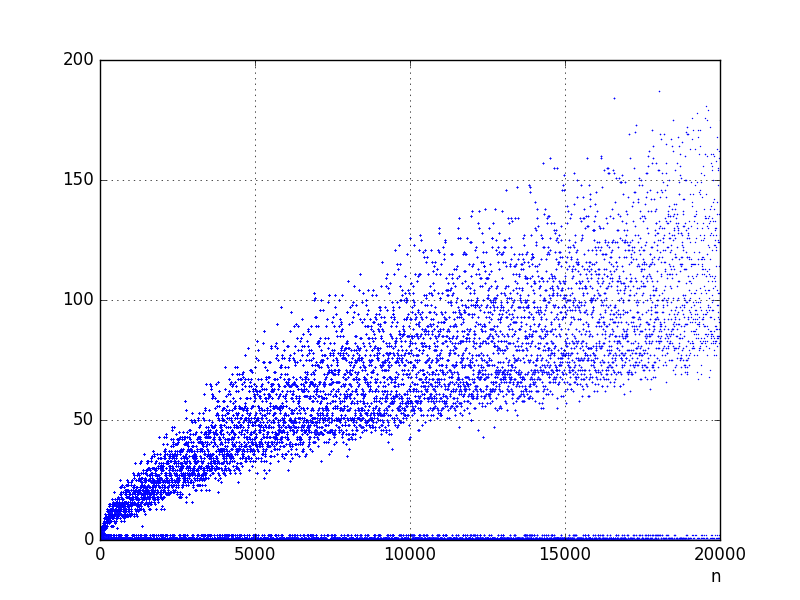
\includegraphics[width=9cm]{f_twin_primes_greater_distinct}
\caption{Number of distinct the greater of twin primes in $R(n)$ ($2$ \textless $n$ \textless $2 \times 10^4$, $n = 2k, k \in \mathbb{N}$)}
\label{fig:greatertwinprime}
\end{figure}

\begin{figure}[!ht]
\centering
\captionsetup{justification=centering}
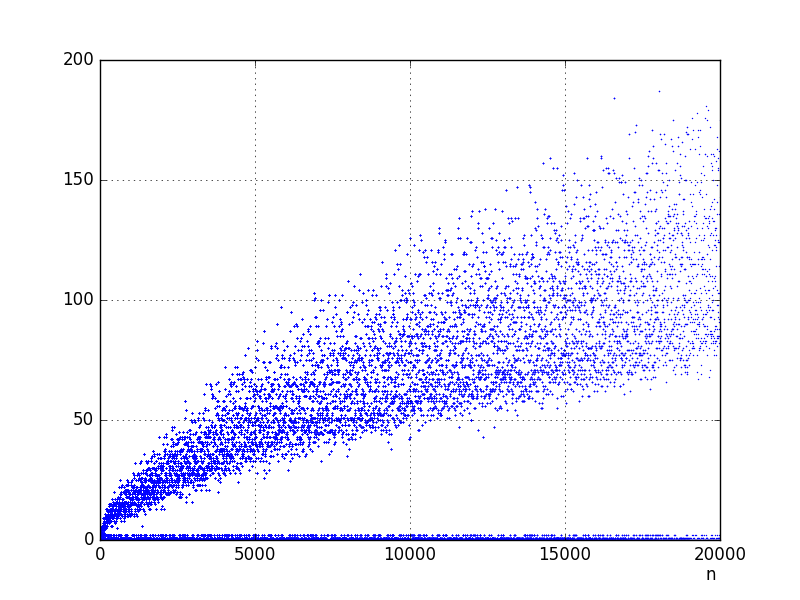
\includegraphics[width=9cm]{f_twin_primes_lesser_distinct}
\caption{Number of distinct the lesser of twin primes in $R(n)$ ($2$ \textless $n$ \textless $2 \times 10^4$, $n = 2k, k \in \mathbb{N}$)}
\label{fig:lessertwinprime}
\end{figure}

Further experiments show that there are in general two categories of even numbers $n$: category 1 - with 0, 1, or 2 distinct greater/lesser of twin primes in all $R(n)$, and category 2 - with fast increasing number of distinct greater/lesser twin primes in $R(n)$  (Figure $\ref{fig:greatertwinprime}$, Figure $\ref{fig:lessertwinprime}$). From all twin primes standpoint such observation is not visible (Figure $\ref{fig:twinprimesall}$) - except $4$ (which has $R(4) = \{(2,2)\}$, without twin primes) even numbers $n$ have at least one twin prime in $R(n)$. Analysis of difference between number of the greater of twin primes and the lesser of twin primes show that there is balance between those two properties of $R(n)$, and average diff is close to $0$ (Figure $\ref{fig:difftwinprimes}$).\par

\begin{figure}[!ht]
\centering
\captionsetup{justification=centering}
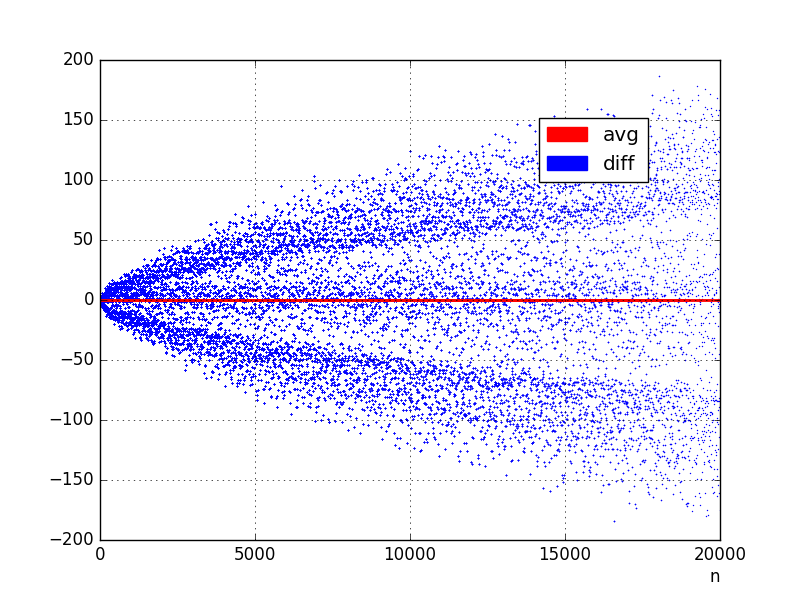
\includegraphics[width=9cm]{f_diff_greater_lesser_twin_primes}
\caption[caption]{Difference (diff) between number of distinct  the greater and the lesser of twin primes in $R(n)$, including average value (avg) ($2$ \textless $n$ \textless $2 \times 10^4$, $n = 2k, k \in \mathbb{N}$)}
\label{fig:difftwinprimes}
\end{figure}

\begin{figure}[!ht]
\centering
\captionsetup{justification=centering}
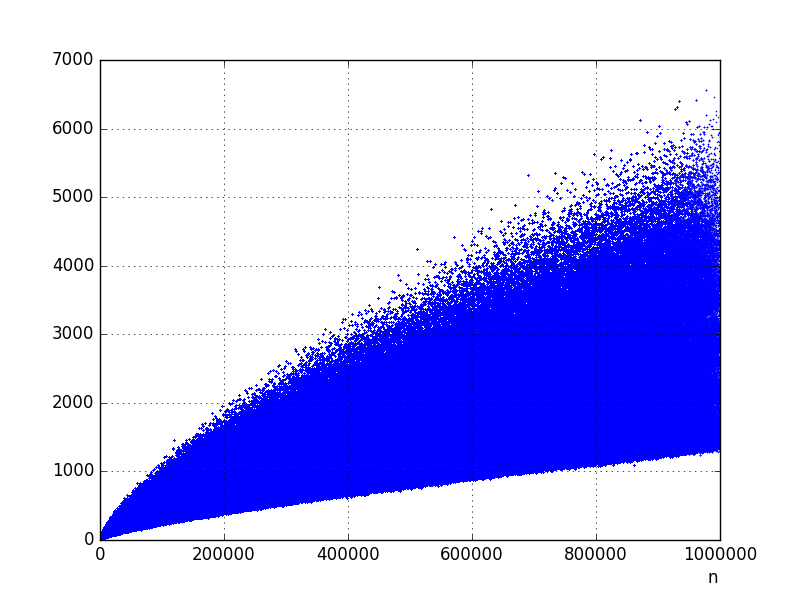
\includegraphics[width=9cm]{f_twin_primes_all}
\caption{Number of distinct twin primes in $R(n)$ \\ ($2$ \textless $n$ \textless $10^6$, $n = 2k, k \in \mathbb{N}$)}
\label{fig:twinprimesall}
\end{figure}

\begin{figure}[!ht]
\centering
\captionsetup{justification=centering}
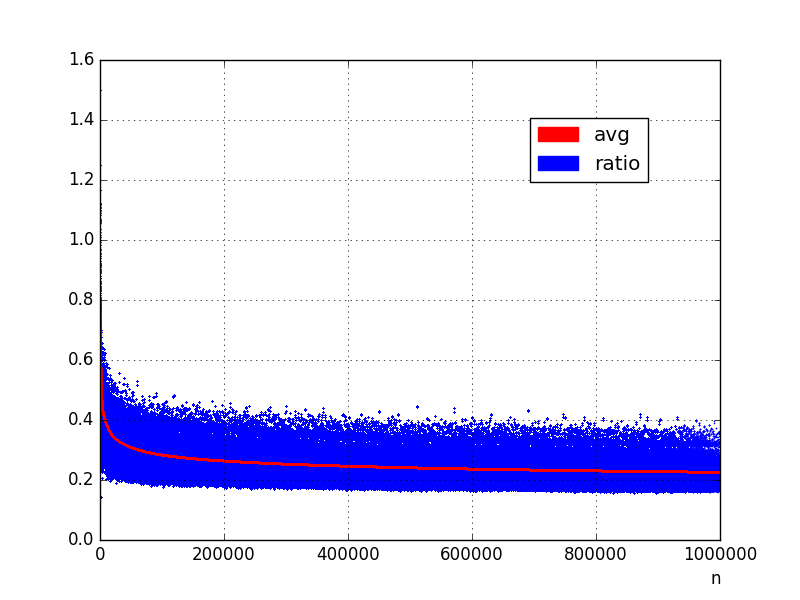
\includegraphics[width=9cm]{f_ratio_twin_primes_to_all_primes}
\caption{$\frac{T(n)}{C(n)}$ (ratio), including its average value (avg) \\ ($2$ \textless $n$ \textless $10^6$, $n = 2k, k \in \mathbb{N}$)}
\label{fig:ratiotwinprimesallpairs}
\end{figure}

Let $T(n)$ be a number of twin primes in all $R(n)$ and $C(n) = \left\vert{R(n)}\right\vert$. Examination of $\frac{T(n)}{C(n)}$ for consecutive even $n$ shows that the sequence has a downward trend (Figure $\ref{fig:ratiotwinprimesallpairs}$). This illustration may be yet another expression of the scarcity of twin primes, like Brun's constant \cite{brun1919}.

\section{Extended strong Goldbach conjecture}

Executed experiments, especially non-zero values observed in Figures $\ref{fig:twinprimesall}$ and $\ref{fig:ratiotwinprimesallpairs}$ let build the hypothesis that strong Goldbach conjecture can be extended from original form (1):

\begin{equation}
\displaystyle\mathop{\bigforall}_{n>1, n \in \mathbb{N}} \displaystyle\mathop{\bigexists}_{p, q \in \mathbb{P}} 2 \times n = p + q
\end{equation}

to the new one (2), skipping just the first case ($n = 2$) for which is not true:

\begin{equation}
\displaystyle\mathop{\bigforall}_{n>2, n \in \mathbb{N}} \displaystyle\mathop{\bigexists}_{p \in \mathbb{P_T}, q \in \mathbb{P}} 2 \times n = p + q
\end{equation}

Stronger version of (2) is not true - assumption (3):

\begin{equation}
\displaystyle\mathop{\bigforall}_{n>2, n \in \mathbb{N}} \displaystyle\mathop{\bigexists}_{p, q \in \mathbb{P_T}} 2 \times n = p + q
\end{equation}

has at least 35 counter-examples, listed in OEIS A007534 \cite{A007534} and evaluated at \cite{zwillinger1979} (and this is still an open question if this list is complete).

\section{Summary and future work}

Although extended strong Goldbach conjecture (2) does not help, directly, in proving the original problem stated by Goldbach and Euler (1), it depicts that there is even greater synergy between sum of primes and consequtive even numbers - twin primes are also important builders of even numbers. As a result of this work three integer sequences were submitted to OEIS database: OEIS A294185 \cite{A294185}, OEIS A294186 \cite{A294186} and OEIS A295424 \cite{A295424}. \par
Additionaly, presented work provides few more interesting questions which can be a foundation of further research work. Is $\displaystyle{\lim_{n \to \infty}}$ $\frac{T(n)}{C(n)}$ converging to a positive number or zero? Is it possible to find a pattern between even numbers for which number of the lesser or the greater of twin primes in $R(n)$ is zero? Why there are two categories of numbers: first one with the $\leq 2$ lesser or the greater of twin primes in $R(n)$, and second one - with the lesser and the greater twin primes $\textgreater 2$, which is growing with $n$?\par

\begin{thebibliography}{9}
\bibitem{goldbach1742}
  Christian Goldbach, 
  \emph{On the margin of a letter to Leonard Euler},
  1742.
\bibitem{oliveira2012}
  Tomás Oliveira e Silva,
  \emph{Goldbach conjecture verification.}
  http://sweet.ua.pt/tos/goldbach.html,
  2012.
\bibitem{oliveira2013}
  Tomás Oliveira e Silva, Siegfried Herzog, and Silvio Pardi, 
  \emph{Empirical verification of the even Goldbach conjecture and computation of prime gaps up to 4 $\times 10^{18}$.}, 
  Mathematics of Computation, vol. 83, no. 288, pp. 2033-2060, 
  July 2014 (published electronically on November 18, 2013.
\bibitem{woon2000}
  Max S.C. Woon,
  \emph{On Partitions of Goldbach's Conjecture}, arXiv:math/0010027 [math.GM], 2000.  
\bibitem{A014574}
  OEIS Foundation Inc. (2018), The On-Line Encyclopedia of Integer Sequences, http://oeis.org/A014574. Average of twin prime pairs.
\bibitem{A001359}
  OEIS Foundation Inc. (2018), The On-Line Encyclopedia of Integer Sequences, http://oeis.org/A001359. Lesser of twin primes.
\bibitem{A006512}
  OEIS Foundation Inc. (2018), The On-Line Encyclopedia of Integer Sequences, http://oeis.org/A294186. Number of distinct greater twin primes which are in Goldbach partitions of 2n.
\bibitem{A294185}
  OEIS Foundation Inc. (2018), The On-Line Encyclopedia of Integer Sequences, http://oeis.org/A006512. Greater of twin primes. 
\bibitem{A294186}
  OEIS Foundation Inc. (2018), The On-Line Encyclopedia of Integer Sequences, http://oeis.org/A294185. Number of distinct lesser twin primes which are in Goldbach partitions of 2n.
\bibitem{A295424}
  OEIS Foundation Inc. (2018), The On-Line Encyclopedia of Integer Sequences, http://oeis.org/A295424. Number of distinct twin primes which are in Goldbach partitions of 2n.
\bibitem{brun1919}
  Viggo Brun,
  \emph{La série 1/5+1/7+1/11+..., où les dénominateurs sont nombres premiers jumeaux est convergente ou finie"},
  Bulletin des Sciences Mathématiques (in French). 43: 100–104, 124–128, 
  1919.
\bibitem{A007534}
  OEIS Foundation Inc. (2018), The On-Line Encyclopedia of Integer Sequences, http://oeis.org/A007534. Even numbers that are not the sum of a pair of twin primes.
\bibitem{zwillinger1979}
  Dan Zwillinger, 
  \emph{A Goldbach Conjecture Using Twin Primes.}
  Math. Comp. 33, No.147, p.1071,
  1979.
  
\end{thebibliography}

\end{document}
